\section{Definiciones y resultados previos}
		\begin{frame}{Lipschitz}		
			\begin{definition}
				Sea $\Omega \subset \mathbb{R}^2$ y sea $f : \Omega \rightarrow \mathbb{R}$. Se dice que $f$ es lipschitziana respecto de la segunda variable, $y$, si existe una constante $L \in \mathbb{R^{+}}$, llamada constante de Lipschitz, de forma que $|f(t,y_1) - f(t, y_2)| \le L|y_1 - y_2|$ para cualquier par de puntos $(t,y_1), (t,y_2) \in \Omega$.  
			\end{definition}
		\end{frame}
	


		\begin{frame}{Existencia y unicidad}
			\fontsize{11}{11}\selectfont
			\begin{theorem} \label{theorem:existence-uniqueness}
				(Existencia y unicidad de soluciones) Sea $f: [a,b] \times I \rightarrow \mathbb{R}$, donde I es un intervalo de $\mathbb{R}$, y sea $y_0 \in I$. Entonces:
				\begin{enumerate}
					\item Si $I = [\alpha,\beta]$ y $f$ es lipschitziana respecto de la segunda variable en $[a,b]\times[\alpha,\beta]$, entonces existe $c \in [a,b]$ tal que el problema de valores iniciales:
					\begin{center}
						$\begin{cases}
						y'(t) = f(t,y(t)) \\
						y(a) = y_0 \\
						t \in [a,c] \\
						\end{cases}$
					\end{center}
					tiene exactamente una solución.
					\item Si $I = ]-\infty,\infty[$ y $f$ es lipschitziana respecto de la segunda variable en $[a,b]\times]-\infty,\infty[$, entonces existe exactamente una solución en $[a,b]$
				\end{enumerate}
			\end{theorem}
		\end{frame}	
			
		\begin{frame}{}		
				\begin{theorem} \label{theorem:desigualdad-sols}
					Sean dos soluciones $y(t), z(t)$ de la ecuación diferencial $y'(t) = f(t,y(t))$ para las condiciones iniciales $y(a)$ y $z(a)$ respectivamente. Supóngase que $f$ es lipschitziana respecto de la segunda variable. Entonces $|y(t)-z(t)| \leq e^{L(t-a)}|y(a)-z(a)|$ donde L es la constante de Lipschitz de $f$.
				\end{theorem}						
		\end{frame}
				
		\begin{frame}{Errores locales y globales}		
			\begin{definition}
				Sean $w_i$ los valores estimados en los puntos $t_i$ por cierto método de discretización. Sea también $z_i$ el valor de la solución exacta en $t_i$ para el problema de valores iniciales
		
				\begin{equation}
					\begin{cases}
					y'(t) = f(t,y(t)) \\
					y(t_{i-1}) = w_{i-1} \\
					t \in [t_{i-1},t_{i}] \\
					\end{cases}
				\end{equation}
		
				Se definen los siguientes errores:
		
				\begin{itemize}
					\item Error global de truncatura o error acumulado en el nodo i-ésimo: $g_i=|y_i - w_i|$
					\item Error local de truncatura o error en un paso: $e_i = |z_i - w_i|$
				\end{itemize}
			\end{definition}				
		\end{frame}
		
		\begin{frame}{Errores locales y globales}		
			\begin{figure}[h]
				\centering
				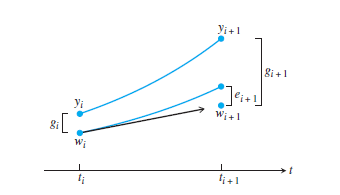
\includegraphics[width=10cm]{./Images/error-euler.png}
				\caption{Representación gráfica de los errores locales y globales.}
				\label{fig:error}
			\end{figure}	
		\end{frame}
		
	
		\begin{frame}{Errores locales y globales}	
			\begin{theorem} \label{theorem:local-global-error}
				Supóngase que la función $f$ es lipschitziana en la segunda variable con constante de Lipschitz $L$. Además, supóngase que existen $C \ge 0$ y $k \in \mathbb{N}$ tales que los errores locales verifican $e_i \le C h^{k+1}$ para todo $i = 0 \ldots n$. Entonces, se verifica la siguiente desigualdad para los errores globales
						
				\begin{equation}
					g_i \le \frac{C h^k}{L} (e^{L(t_i-a)}-1)
				\end{equation}
			\end{theorem}
		\end{frame}	 
		
		\begin{frame}{Método de discretización}
			\fontsize{11}{11}\selectfont
			\begin{definition}
				Considérese un método de discretización para problemas de valores iniciales. Entonces:
				\begin{enumerate}
					\item El método es localmente de orden $k$ si existe una constante $C \ge 0$ tal que $e_i \le C h^k$ para todo $i = 0 \ldots n$ cuando h tiende a 0.
					\item El método es de orden $k$ si existe una constante $C \ge 0$ tal que $g_i \le C h^k$ para todo $i = 0 \ldots n$ cuando h tiende a 0.
				\end{enumerate}
			\end{definition}
			
			\begin{theorem} \label{theorem:euler:error}
				Supóngase que $f: [a,b] \times [\alpha, \beta] \rightarrow \mathbb{R}$ es derivable y lipschitziana en la segunda variable. Entonces, el método de Euler es localmente de orden $2$. Consecuentemente, el método de Euler es de orden $1$.
			\end{theorem}	
		\end{frame}
			
		\begin{frame}{Método de discretización}		
			\begin{definition}
			Un método de un paso se dice convergente respecto a la ecuación diferencial que aproxima (con función $f$ lipschitziana con respecto a la segunda variable) si:
			$$ \lim_{n \rightarrow +\infty} \max_{i = 0 \ldots n} g_i = 0 $$
			\end{definition}
	
		    \begin{definition}
		    	Un método de un paso se dice consistente con respecto a la ecuación diferencial que aproxima (con función $f$ lipschitziana con respecto a la segunda variable) si:
		    	$$ \lim_{n \rightarrow +\infty} \max_{i = 0 \ldots n} e_i = 0 $$
		    	Esto es, los errores locales convergen uniformemente a 0 cuando $n \rightarrow +\infty$.
		    \end{definition}
		\end{frame}	
			
		\begin{frame}{Método de discretización}
			\begin{definition}
				Un método de discretización se dice estable si para cualquier PVI verificando que $f$ es lipschitziana respecto de la segunda variable y para cualquier perturbación de este PVI existen constantes positivas $h_0$ y $K$ tales que la diferencia entre las aproximaciones obtenidas para ambos PVI están acotadas por $K |y_0 - y'_0|$ para todo $h \in [0,h_0]$. Esto es, si $w_i$ son las aproximaciones obtenidas para el problema sin perturbar y $w'_i$ son las aproximaciones obtenidas para el problema perturbado, utilizando en ambos casos el mismo $h < h_0$, entonces $\left|w_i - w'_i\right| \le K |y_0 - y'_0|$ para todo $i$.
			\end{definition}
		\end{frame}
		
		\begin{frame}{Estabilidad y convergencia}
			\begin{theorem}
				Si un método de un paso anterior verifica que $\phi$ es continua en cada una de sus variables y, además, es lipschitziana respecto de la segunda variable en el correspondiente dominio para $h \in [0, h_0]$, entonces:
				
				\begin{enumerate}
					\item el método es estable.
					\item el método es convergente o, equivalentemente, $\phi(b,y,0) = f(b,y)$.
				\end{enumerate}
			\end{theorem}
		\end{frame}